\documentclass[runningheads]{llncs}
\usepackage[T1]{fontenc}
\usepackage{amsmath,amssymb}
\usepackage{xcolor}
\usepackage{tikz-cd}
\usetikzlibrary{decorations.pathreplacing}
\usetikzlibrary{decorations.markings,arrows.meta}
\usetikzlibrary{fit,backgrounds}
\tikzset{
	midarrow/.style={
		postaction={
		decorate,
		decoration={markings,mark=at position 0.9 with {\arrow{>[length=6pt,width=6pt]}}}
		}
	}
}

\begin{document}

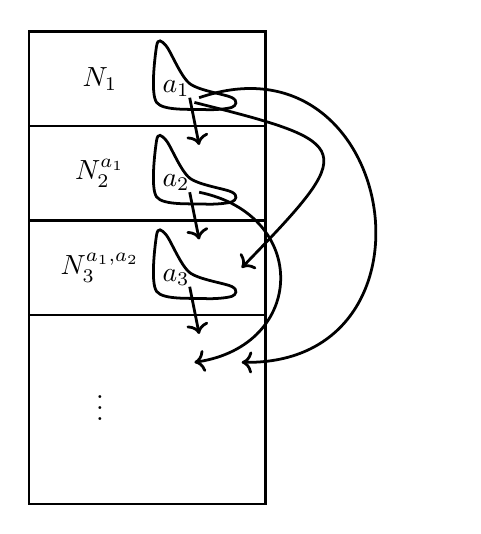
\begin{tikzpicture}[scale=0.6,line width=1pt]
\draw (0,0) rectangle (5,10);
\draw (0,4) -- (5,4);
\draw (0,6) -- (5,6);
\draw (0,8) -- (5,8);
\node at (1.5,9) {$N_1$};
\node at (1.5,7) {$N_2^{a_1}$};
\node at (1.5,5) {$N_3^{a_1,a_2}$};
\node at (1.5,2.2) {$\vdots$};
%
\node[right] at (2.6,8.8) {$a_1$};
\draw plot [smooth cycle] coordinates {
    (2.7,8.5)
    (3.7,8.35)
    (4.3,8.4)
    (4.3,8.6)
    (3.4,8.9)
    (2.9,9.7)
    (2.7,9.7)
};
\draw[->] (3.4,8.6) -- (3.6,7.6);
\draw[->] (3.5,8.5) to[bend left=60, looseness=2.5] (4.5,5);
\draw[->] (3.6,8.6) to[bend left=100, looseness=2] (4.5,3);
\node[right] at (2.6,6.8) {$a_2$};
\draw plot [smooth cycle] coordinates {
    (2.7,6.5)
    (3.7,6.35)
    (4.3,6.4)
    (4.3,6.6)
    (3.4,6.9)
    (2.9,7.7)
    (2.7,7.7)
};
\draw[->] (3.4,6.6) -- (3.6,5.6);
\draw[->] (3.6,6.6) to[bend left=80, looseness=1.7] (3.5,3);
\node[right] at (2.6,4.8) {$a_3$};
\draw plot [smooth cycle] coordinates {
    (2.7,4.5)
    (3.7,4.35)
    (4.3,4.4)
    (4.3,4.6)
    (3.4,4.9)
    (2.9,5.7)
    (2.7,5.7)
};
\draw[->] (3.4,4.6) -- (3.6,3.6);
\end{tikzpicture}

\end{document}